\datos{color}{}{}

\subsection{\textit{Unitree G1}}

El \textit{Unitree G1}, Figura \ref{unitreeg1}, es un robot humanoide desarrollado por \textit{Unitree Robotics} a partir de 
2021 como plataforma de investigación en locomoción bípeda, manipulación y control dinámico. 
Su diseño compacto y ligero, junto con actuadores de alto par y sensores avanzados, lo 
convierten en un humanoide adecuado para tareas de navegación autónoma, interacción con 
objetos y experimentación en entornos reales. Su diseño modular permite integrar sensores adicionales, cámaras 
\textit{RGB-D}, \textit{LiDAR 3D} y herramientas de manipulación, adaptándose a múltiples escenarios de 
investigación y aplicaciones reales. \\\\

Sus usos principales incluyen la investigación en locomoción bípeda, control predictivo, 
aprendizaje por refuerzo, manipulación autónoma, interacción humano–robot y aplicaciones 
industriales ligeras. También se emplea como plataforma educativa y experimental en 
laboratorios de robótica humanoide debido a su coste relativamente bajo y su arquitectura 
abierta a nivel de software. \\

La arquitectura del \textit{G1} es híbrida: un ordenador central ejecuta la percepción,
la planificación de movimientos y la supervisión del sistema, mientras que cada 
articulación incorpora controladores locales responsables del control de par, posición y 
estabilidad. La comunicación entre módulos se realiza mediante buses de alta velocidad y 
\textit{ROS2}, integrando percepción, locomoción y manipulación en un sistema distribuido. \\

\begin{wrapfigure}{r}{0.4\textwidth}
    \centering
    \vspace{-10pt}
    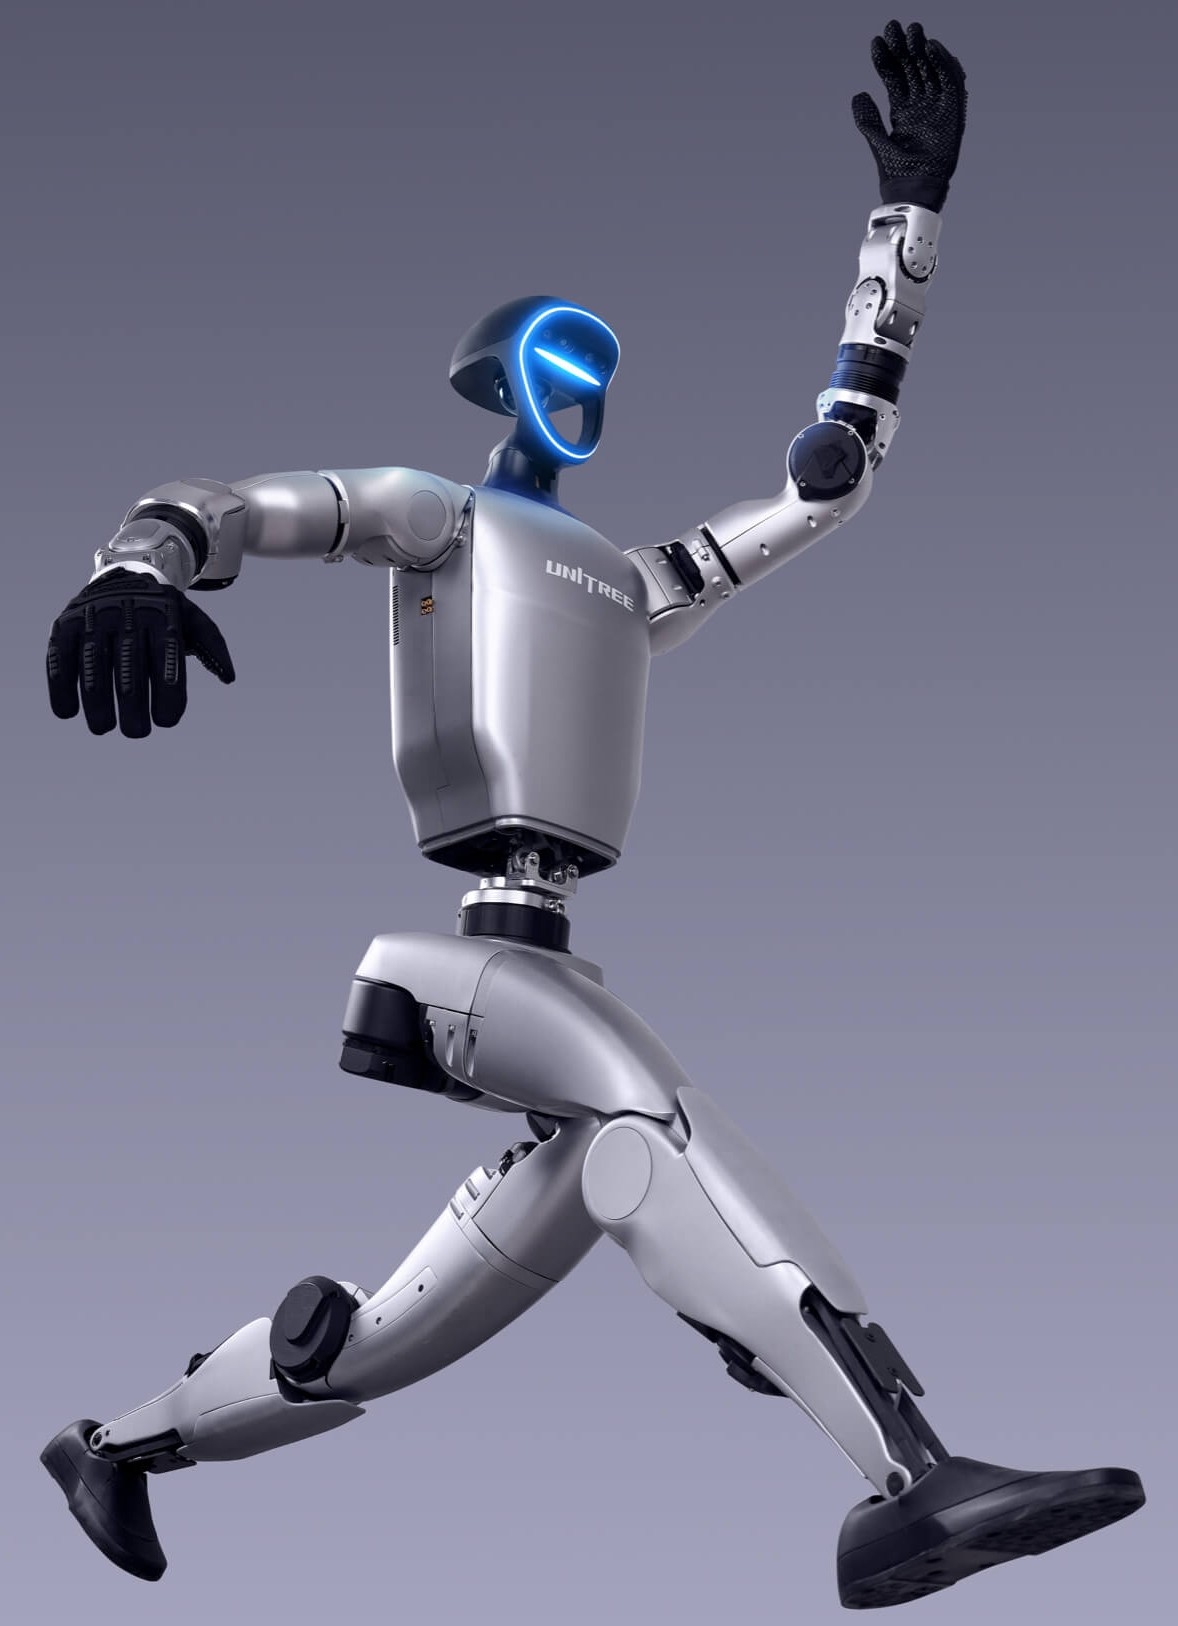
\includegraphics[width=0.2\textwidth]{Images/unitreeG1.jpg}
    \caption{\textit{Unitree G1}.}
    \label{unitreeg1}
    \vspace{-10pt}
\end{wrapfigure}

El método de locomoción se basa en dos piernas articuladas con múltiples grados de libertad, 
accionadas por motores eléctricos de alta potencia y controladas mediante algoritmos de 
control dinámico basados en modelos del centro de masa y control predictivo. Esta 
configuración permite caminar, mantener el equilibrio ante perturbaciones y ejecutar 
movimientos ágiles. El robot puede equiparse con manos robóticas para tareas de 
manipulación. \\

\subsection*{Referencias}

\cite{UnitreeG1Ref} \fullcite{UnitreeG1Ref}.
